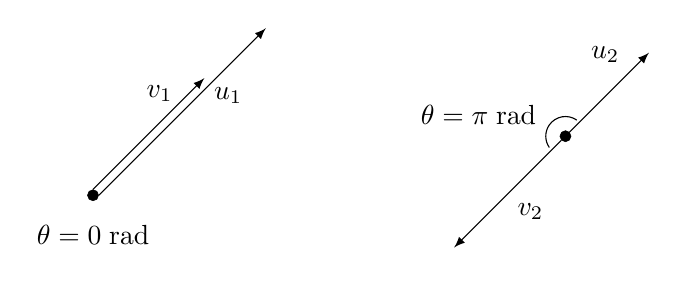
\begin{tikzpicture}[
	point/.style={circle,draw,very thin,fill,inner sep=0pt,minimum size=4pt},
	vector/.style={-latex},
]
	\node[point] at (0,0) (o) {};
	\draw[vector] (o.north) to node[below right,at end] {$\uvec{u}_1$} ++(45:2cm);
	\draw[vector] (o.east) to node[above left] {$\uvec{v}_1$} ++(45:3cm);
	\node at (0,-0.5) {$\theta = 0\;\mathrm{rad}$};
	\begin{scope}[xshift=6cm,yshift=0.75cm]
		\node[point] at (0,0) (o) {};
		\draw[vector] (o) to node[above left, near end] {$\uvec{u}_2$} ++(45:1.5cm);
		\draw[vector] (o) to node[below right] {$\uvec{v}_2$} ++(225:2cm);
		%	\node at (0.5,0) {$\theta = \pi\;\mathrm{rad}$};
		\draw ([shift=(55:0.25cm)]0,0) arc (55:215:0.25cm) node[above left,near end]
			{$\theta = \pi\;\mathrm{rad}$};
	\end{scope}
\end{tikzpicture}
